% =============================================================================
%  ACI Companion — Session 6: Ant Colony Optimization & Neural Architecture Search
%  Generated from CS6.pdf (AIMLCZG557, BITS Pilani)
%  Build: pdflatex adversarial-search.tex && pdflatex adversarial-search.tex
% =============================================================================

\documentclass[a4paper,11pt]{article}

% ---- Encoding & fonts -------------------------------------------------------
\usepackage[T1]{fontenc}
\usepackage[utf8]{inputenc}
\usepackage{lmodern}
\usepackage{microtype}

% ---- Geometry ---------------------------------------------------------------
\usepackage[a4paper,margin=1in,headheight=15pt,headsep=14pt]{geometry}

% ---- Math -------------------------------------------------------------------
\usepackage{amsmath,amssymb}

% ---- Graphics, tables, colour -----------------------------------------------
\usepackage{graphicx}
\usepackage{booktabs}
\usepackage[table,svgnames]{xcolor}
\usepackage{adjustbox}

% ---- Callout boxes ----------------------------------------------------------
\usepackage[most]{tcolorbox}
\tcbuselibrary{skins,breakable}

% ---- Tikz (inline diagrams) -------------------------------------------------
\usepackage{tikz}
\usetikzlibrary{arrows.meta,positioning,shapes.geometric,calc}

% ---- Callout glyphs ---------------------------------------------------------
\usepackage{pifont}
\IfFileExists{bbding.sty}{%
  \usepackage{bbding}%
  \newcommand{\glyphHand}{\HandRight}%
  \newcommand{\glyphPencil}{\PencilRight}%
}{%
  \newcommand{\glyphHand}{\ding{43}}%
  \newcommand{\glyphPencil}{\ding{46}}%
}

% ---- Lists & spacing --------------------------------------------------------
\usepackage{enumitem}
\setlist{leftmargin=1.5em,topsep=4pt,itemsep=3pt}

% ---- Dedicated steps list for worked examples --------------------------------
\newlist{steps}{enumerate}{1}
\setlist[steps]{label=\textbf{Step \arabic*.},
  leftmargin=4.4em, labelwidth=3.8em, labelsep=0.6em, labelindent=0pt,
  align=left, topsep=5pt, itemsep=6pt}

\usepackage{parskip}

% ---- Headers / footers ------------------------------------------------------
\usepackage{fancyhdr}

% ---- Section styling --------------------------------------------------------
\usepackage{titlesec}

% ---- Links ------------------------------------------------------------------
\usepackage[hidelinks]{hyperref}
\usepackage{xurl}
\hypersetup{breaklinks=true}

% =============================================================================
%  COLOURS
% =============================================================================
\definecolor{navy}{HTML}{21355E}
\definecolor{navyrule}{HTML}{21355E}
\definecolor{inktext}{HTML}{1A202C}
\definecolor{mutedtext}{HTML}{6B7280}

\definecolor{intuFrame}{HTML}{2C5AA0}   \definecolor{intuFill}{HTML}{F4F7FC}
\definecolor{everyFrame}{HTML}{8A5A1E}  \definecolor{everyFill}{HTML}{FBF1E3}
\definecolor{workFrame}{HTML}{2E7D52}   \definecolor{workFill}{HTML}{F1F8F3}
\definecolor{watchFrame}{HTML}{B23A48}  \definecolor{watchFill}{HTML}{FBF1F2}
\definecolor{keyFrame}{HTML}{6A4C93}    \definecolor{keyFill}{HTML}{F4F0F9}

\color{inktext}
\hypersetup{linkcolor=navy,urlcolor=navy,citecolor=navy}

% =============================================================================
%  RUNNING HEADER / FOOTER
% =============================================================================
\newcommand{\CourseShort}{ACI Companion}
\newcommand{\SessionNo}{6}
\newcommand{\LectureTitle}{ACO \& Neural Architecture Search}

\pagestyle{fancy}
\fancyhf{}
\fancyhead[L]{\footnotesize\color{mutedtext}\textsf{\CourseShort}}
\fancyhead[R]{\footnotesize\color{mutedtext}\textsf{Session \SessionNo\ \textperiodcentered\ \LectureTitle}}
\fancyfoot[C]{\footnotesize\color{mutedtext}\thepage}
\renewcommand{\headrulewidth}{0.4pt}
\renewcommand{\footrulewidth}{0pt}
\renewcommand{\headrule}{\hbox to\headwidth{\color{navyrule!55}\leaders\hrule height \headrulewidth\hfill}}

% =============================================================================
%  SECTION HEADINGS
% =============================================================================
\titleformat{\section}
  {\sffamily\Large\bfseries\color{navy}}
  {\thesection}{0.8em}{}
  [{\vspace{2pt}\color{navy!70}\titlerule[0.8pt]}]
\titleformat{\subsection}
  {\sffamily\large\bfseries\color{navy!92}}
  {\thesubsection}{0.7em}{}
\titlespacing*{\section}{0pt}{16pt}{8pt}
\titlespacing*{\subsection}{0pt}{12pt}{4pt}

% =============================================================================
%  PILL-TAB CALLOUT BOXES
% =============================================================================
\tcbset{
  housecallout/.style 2 args={
    enhanced, breakable,
    colback=#2, colframe=#1,
    boxrule=0.6pt, arc=2.4pt, outer arc=2.4pt,
    left=10pt, right=10pt, top=9pt, bottom=9pt,
    before skip=11pt, after skip=11pt,
    fontupper=\normalsize,
    coltitle=white,
    fonttitle=\bfseries\sffamily\small,
    attach boxed title to top left={xshift=6mm,yshift=-3mm},
    boxed title style={
      colback=#1, colframe=#1,
      rounded corners, arc=3pt,
      boxrule=0pt, left=6pt, right=6pt, top=2pt, bottom=2pt
    }
  }
}

\newtcolorbox{intuition}{%
  housecallout={intuFrame}{intuFill},
  title={\raisebox{-0.05ex}{\glyphHand}\,\ The intuition}}

\newtcolorbox{everyday}{%
  housecallout={everyFrame}{everyFill},
  title={\raisebox{-0.05ex}{$\bigstar$}\,\ Everyday picture}}

\newtcolorbox{worked}[1]{%
  housecallout={workFrame}{workFill},
  title={\raisebox{-0.05ex}{\glyphPencil}\,\ Worked example: #1}}

\newtcolorbox{watchout}{%
  housecallout={watchFrame}{watchFill},
  title={\raisebox{-0.05ex}{\ding{55}}\,\ Watch out}}

\newtcolorbox{keytake}{%
  housecallout={keyFrame}{keyFill},
  title={\raisebox{-0.05ex}{\ding{51}}\,\ Key takeaway}}

% =============================================================================
%  TITLE BANNER
% =============================================================================
\providecommand{\addfontfeatureslike}[1]{#1}
\newcommand{\titlebanner}[4]{%
  \begin{tcolorbox}[
    enhanced, breakable=false,
    colback=navy, colframe=navy,
    boxrule=0pt, arc=3pt, outer arc=3pt,
    left=16pt, right=16pt, top=16pt, bottom=16pt,
    before skip=2pt, after skip=14pt,
    width=\linewidth ]
    {\sffamily\footnotesize\bfseries\color{white!85}%
      \MakeUppercase{\addfontfeatureslike{#1}}}\par
    \vspace{6pt}
    {\sffamily\bfseries\fontsize{26}{30}\selectfont\color{white} #2\par}
    \vspace{5pt}
    {\sffamily\large\color{white!88} #3\par}
    \vspace{9pt}
    {\color{white!55}\rule{\linewidth}{0.4pt}}\par
    \vspace{6pt}
    {\sffamily\footnotesize\color{white!82} #4\par}
  \end{tcolorbox}%
}

% =============================================================================
%  \housefig
% =============================================================================
\newcommand{\housefig}[2]{%
  \begin{figure}[htbp]
    \centering
    \includegraphics[width=\linewidth]{#1}%
    \caption{#2}
  \end{figure}%
}

\newcommand{\vocab}[1]{\textbf{\color{navy}#1}}

% =============================================================================
\begin{document}
% =============================================================================

\thispagestyle{fancy}

\titlebanner
  {ACI Companion Reader \textperiodcentered\ AIMLCZG557}
  {Ant Colony Optimization \& Neural Architecture Search}
  {Session 6 --- From swarm intelligence to self-designing AI}
  {Session 6 \textperiodcentered\ Read alongside the lecture slides \textperiodcentered\ Every slide example worked out in full}

\noindent\textbf{How to use this companion.}
The slides give you the formulas; this reader gives you the \emph{why}.
Every slide concept is expanded into a plain-English explanation.
Every slide example is worked out step by step.
Five box types guide you through each concept.
The \textcolor{intuFrame}{\textbf{blue}} box states the core idea.
The \textcolor{everyFrame}{\textbf{amber}} box ties it to real life before any math.
The \textcolor{workFrame}{\textbf{green}} box solves a problem with real numbers.
The \textcolor{watchFrame}{\textbf{red}} box flags the common mistake.
The \textcolor{keyFrame}{\textbf{purple}} box is the one line to remember.

\medskip

% =============================================================================
\section{What this session covers}
% =============================================================================

This session has two big parts.

\begin{enumerate}
  \item \textbf{Ant Colony Optimization (ACO).}
        We look at how simulated ants, leaving digital scent trails, can
        solve hard routing problems like the Travelling Salesman Problem.
  \item \textbf{Neural Architecture Search (NAS) and CoDeepNEAT.}
        We ask: can a computer design its own neural networks?
        The answer is yes --- using evolution.
        We trace the lineage from plain NEAT, through DeepNEAT, to
        CoDeepNEAT, and run through a full worked example.
\end{enumerate}

% =============================================================================
\section{Ant Colony Optimization: the big idea}
% =============================================================================

How do you find the shortest path through a city when there are too many
routes to check one by one?
Real ants solved this problem long before computers existed.

\begin{intuition}
\vocab{ACO} (Ant Colony Optimization) is a search algorithm inspired by
how real ants find food.
Each artificial ant builds a candidate solution.
It leaves a chemical signal, called a \vocab{pheromone}, on the path it
took.
Good paths collect more pheromone.
Over many rounds, the colony converges on the best route.
\end{intuition}

\begin{everyday}
Imagine a food court with many corridors.
Hundreds of people walk from the entrance to the counter.
Some try the long route; some try the shortcut.
People notice the crowds ahead and tend to follow the busier path.
The short, fast corridor gets more foot traffic.
Over time almost everyone uses it.
That is pheromone in human form.
\end{everyday}

% ACO pheromone loop diagram
\begin{figure}[htbp]
\centering
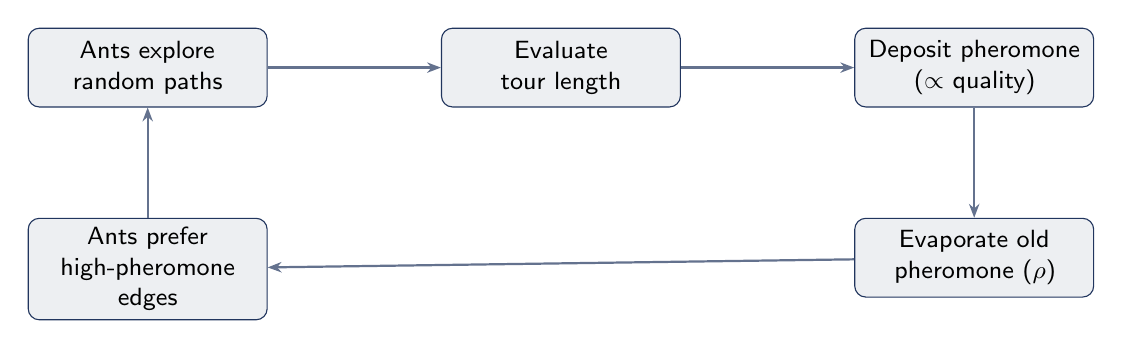
\begin{tikzpicture}[
  node distance=2.2cm,
  box/.style={rectangle,rounded corners=4pt,draw=navy,fill=navy!8,
              text width=2.8cm,align=center,font=\small\sffamily,
              minimum height=1.0cm},
  arr/.style={-{Stealth[length=5pt]},thick,color=navy!70}
]
  \node[box] (ants)   {Ants explore\\ random paths};
  \node[box, right=of ants] (score)  {Evaluate\\ tour length};
  \node[box, right=of score] (update) {Deposit pheromone\\ ($\propto$ quality)};
  \node[box, below=1.4cm of update] (evap)  {Evaporate old\\ pheromone ($\rho$)};
  \node[box, below=1.4cm of ants]  (bias)  {Ants prefer\\ high-pheromone\\ edges};

  \draw[arr] (ants)   -- (score);
  \draw[arr] (score)  -- (update);
  \draw[arr] (update) -- (evap);
  \draw[arr] (evap)   -- (bias);
  \draw[arr] (bias)   -- (ants);
\end{tikzpicture}
\caption*{\small\color{mutedtext}The ACO feedback loop: good routes earn more pheromone, attracting future ants, while evaporation prevents early lock-in.}
\end{figure}

\subsection{ACO parameters}

Every ACO run uses a handful of numbers.
Knowing what each one does lets you tune the algorithm.

\medskip
\begin{adjustbox}{max width=\linewidth}
\begin{tabular}{@{}p{1.6cm}p{3.5cm}p{8cm}@{}}
\toprule
\textbf{Symbol} & \textbf{Name} & \textbf{What it controls} \\
\midrule
$N$           & Number of ants     & Total ants per iteration; $N > 1$ \\
$\tau_0$      & Initial pheromone  & Starting scent on every edge; set to 0 \\
$\tau_{ij}$   & Pheromone on $(i,j)$ & Accumulated scent on the edge from city $i$ to $j$ \\
$\eta_{ij}$   & Heuristic value    & $1/d_{ij}$; short edges get high $\eta$ \\
$\alpha$      & Pheromone weight   & How strongly ants follow scent ($\alpha > 0$) \\
$\beta$       & Distance weight    & How strongly ants prefer short edges ($\beta > 0$) \\
$\rho$        & Evaporation rate   & How fast scent fades; $0 < \rho < 1$ \\
$\text{visit}_k$ & Visit list of ant $k$ & Cities ant $k$ has already visited \\
$Q$           & Pheromone constant & Scales the reward deposited on a completed tour \\
$f_k$         & Tour cost of ant $k$ & Total distance ant $k$ travelled \\
\bottomrule
\end{tabular}
\end{adjustbox}

\subsection{ACO steps}

The algorithm runs three phases per iteration.

\medskip
\noindent\textbf{Initialization.}
Place all $N$ ants at the starting city.
Set $\alpha$, $\beta$, $\rho$.
Set $\tau_0 = 0$ on every edge.

\medskip
\noindent\textbf{Construction.}
Each ant picks its next city using the
\vocab{Next Transition Probability (NTP)}.
For ant $k$ currently at city $i$, the probability of moving to city $j$ is:

\begin{equation}
  NTP_{ij} = \frac{(\tau_{ij})^{\alpha}\,(\eta_{ij})^{\beta}}
               {\displaystyle\sum_{h \notin \text{visit}_k}
                (\tau_{ih})^{\alpha}\,(\eta_{ih})^{\beta}}
\end{equation}

Read it in two pieces.
The numerator scores city $j$: pheromone on that edge to the power
$\alpha$, times the heuristic (inverse distance) to the power $\beta$.
The denominator sums the same score over every city not yet visited.
Dividing gives a probability that sums to 1 over all unvisited cities.

\medskip
\noindent\textbf{Pheromone update.}
After all ants finish their tours, each edge is updated:

\begin{equation}
  \tau_{ij}^{\text{new}} = (1 - \rho)\,\tau_{ij}^{\text{old}} + \Delta\tau_{ij}^{k}
\end{equation}

The term $(1-\rho)\,\tau_{ij}^{\text{old}}$ decays the old scent.
The term $\Delta\tau_{ij}^{k}$ is the fresh deposit by ant $k$:

\begin{equation}
  \Delta\tau_{ij}^{k} =
  \begin{cases}
    Q/f_k & \text{if ant } k \text{ used edge } (i,j) \\
    0      & \text{otherwise}
  \end{cases}
\end{equation}

Ants that completed short tours (small $f_k$) deposit more pheromone per
edge because $Q/f_k$ is large.
That is the positive feedback: good routes attract more future ants.

\begin{watchout}
ACO stops after a fixed number of iterations.
If that limit is reached before an ant completes its tour, the ant is
``dropped'' and its partial path is discarded.
Set the iteration limit generously, or add a completion check before
stopping.
\end{watchout}

\textbf{Where this shows up in ML.}
ACO is used to tune neural network hyperparameters, select features, and
route data in communication networks.
This update works like a reward signal in reinforcement learning.
Edges used by successful agents grow stronger.
This mirrors how actions that led to high reward get reinforced.

\begin{keytake}
ACO replaces exhaustive search with collective learning.
Short, cheap paths collect more pheromone and attract more ants.
Evaporation stops the algorithm from locking onto a suboptimal route early.
\end{keytake}

% =============================================================================
\section{Worked example: Travelling Salesman with ACO}
% =============================================================================

The \vocab{Travelling Salesman Problem} (TSP) is a classic routing puzzle.
You have $n$ cities with known distances between every pair.
Find the shortest tour that visits each city exactly once and returns to the start.

\noindent\textbf{Setup.}
Cities: 1, 2, 3, 4, 5.
Ants $N = 5$ (one per city).
Start city: 4.
Parameters: $\alpha = 0.5$, $\beta = 0.75$, $\rho = 0.1$, $Q = 100$.

\medskip
The distance matrix $d_{ij}$ (symmetric):

\begin{center}\small
\begin{tabular}{@{}c|ccccc@{}}
\toprule
      & 1  & 2  & 3  & 4  & 5  \\
\midrule
1     & 0  & 65 & 52 & 69 & 72 \\
2     & 65 & 0  & 39 & 28 & 43 \\
3     & 52 & 39 & 0  & 72 & 62 \\
4     & 69 & 28 & 72 & 0  & 49 \\
5     & 72 & 43 & 62 & 49 & 0  \\
\bottomrule
\end{tabular}
\end{center}

Initial pheromone values (given in the slides):

\begin{center}\small
\begin{tabular}{@{}llllll@{}}
\toprule
$\tau_{12}=\tau_{21}=0.54$ &
$\tau_{23}=\tau_{32}=0.53$ &
$\tau_{35}=\tau_{53}=0.90$ \\
$\tau_{13}=\tau_{31}=0.53$ &
$\tau_{24}=\tau_{42}=0.39$ &
$\tau_{45}=\tau_{54}=0.68$ \\
$\tau_{14}=\tau_{41}=0.35$ &
$\tau_{25}=\tau_{52}=0.18$ & \\
$\tau_{15}=\tau_{51}=0.24$ &
$\tau_{34}=\tau_{43}=0.32$ & \\
\bottomrule
\end{tabular}
\end{center}

% 5-city TSP network: cities arranged in a rough pentagon, optimal tour highlighted
\begin{figure}[htbp]
\centering
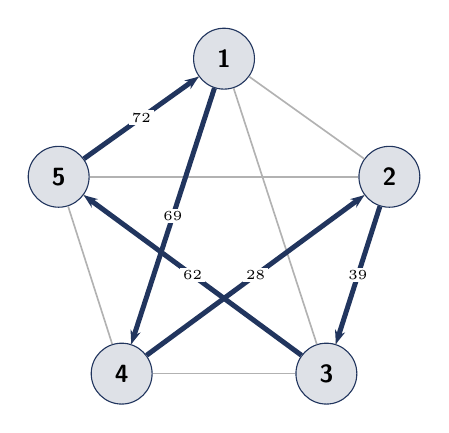
\begin{tikzpicture}[
  city/.style={circle,draw=navy,fill=navy!15,minimum size=22pt,
               font=\small\bfseries\sffamily},
  edge/.style={gray!60,line width=0.6pt},
  tour/.style={navy,line width=1.8pt,-{Stealth[length=5pt]}}
]
  % Place 5 cities at pentagon vertices (approx)
  \node[city] (c1) at (0,2.2)  {1};
  \node[city] (c2) at (2.1,0.7) {2};
  \node[city] (c3) at (1.3,-1.8){3};
  \node[city] (c4) at (-1.3,-1.8){4};
  \node[city] (c5) at (-2.1,0.7){5};

  % All background edges (faint)
  \foreach \a/\b in {c1/c2,c1/c3,c1/c4,c1/c5,c2/c3,c2/c4,c2/c5,c3/c4,c3/c5,c4/c5}{
    \draw[edge] (\a) -- (\b);
  }

  % Optimal tour 4->2->3->5->1->4 in bold navy with arrows
  \draw[tour] (c4) -- (c2);
  \draw[tour] (c2) -- (c3);
  \draw[tour] (c3) -- (c5);
  \draw[tour] (c5) -- (c1);
  \draw[tour] (c1) -- (c4);

  % Distance labels on tour edges
  \node[font=\tiny,fill=white,inner sep=1pt] at ($(c4)!0.5!(c2)$) {28};
  \node[font=\tiny,fill=white,inner sep=1pt] at ($(c2)!0.5!(c3)$) {39};
  \node[font=\tiny,fill=white,inner sep=1pt] at ($(c3)!0.5!(c5)$) {62};
  \node[font=\tiny,fill=white,inner sep=1pt] at ($(c5)!0.5!(c1)$) {72};
  \node[font=\tiny,fill=white,inner sep=1pt] at ($(c1)!0.5!(c4)$) {69};
\end{tikzpicture}
\caption*{\small\color{mutedtext}The 5-city TSP network. Bold arrows show the tour the ant finds: $4\to2\to3\to5\to1\to4$, total distance 270.}
\end{figure}

\begin{worked}{TSP step 1 --- move from city 4}
The ant starts at city 4.
Unvisited cities: 1, 2, 3, 5.
We compute $NTP_{4j}$ for each.

$\eta_{4j} = 1/d_{4j}$, raised to power $\beta = 0.75$.
Each numerator is $(\tau_{4j})^{0.5} \cdot (1/d_{4j})^{0.75}$.

\begin{steps}
  \item \textbf{Compute each numerator.}
        \begin{align*}
          \text{To city 1:} & \quad (0.35)^{0.5} \cdot (1/69)^{0.75} = 0.0247 \\
          \text{To city 2:} & \quad (0.39)^{0.5} \cdot (1/28)^{0.75} = 0.0513 \\
          \text{To city 3:} & \quad (0.32)^{0.5} \cdot (1/72)^{0.75} = 0.0229 \\
          \text{To city 5:} & \quad (0.68)^{0.5} \cdot (1/49)^{0.75} = 0.0445
        \end{align*}

  \item \textbf{Sum the numerators (denominator).}
        \[
          D = 0.0247 + 0.0513 + 0.0229 + 0.0445 = 0.1434
        \]

  \item \textbf{Compute each probability.}
        \begin{align*}
          P_{41} &= 0.0247 / 0.1434 = 0.1723 \\
          P_{42} &= 0.0513 / 0.1434 = \mathbf{0.3577} \\
          P_{43} &= 0.0229 / 0.1434 = 0.1596 \\
          P_{45} &= 0.0445 / 0.1434 = 0.3104
        \end{align*}

  \item \textbf{Pick the next city.}
        $P_{42}$ is largest.
        The ant moves from city 4 to city \textbf{2}.
        $\text{visit}_k = [4, 2]$.

  \item \textbf{Update pheromone on edge (4,2).}
        Deposit: $\Delta\tau_{42} = Q/d_{42} = 100/28 = 3.571$.
        \[
          \tau_{42}^{\text{new}}
            = (1 - 0.1) \times 0.39 + 3.571 = 0.351 + 3.571 = \mathbf{3.922}
        \]
        All other edges simply evaporate by factor $0.9$.
        For example: $\tau_{12}^{\text{new}} = 0.9 \times 0.54 = 0.486$.

  \item \textbf{Sense-check.}
        Edge $(4,2)$ is the shortest from city 4 ($d = 28$).
        It should have the highest probability and it does.
\end{steps}
\end{worked}

\begin{worked}{TSP step 2 --- move from city 2 (visit: 4-2)}
Unvisited: cities 1, 3, 5.
Updated pheromones after step 1:
$\tau_{12} = 0.486$, $\tau_{23} = 0.477$, $\tau_{25} = 0.162$.

\begin{steps}
  \item \textbf{Compute numerators from city 2.}
        \begin{align*}
          \text{To 1:} & \quad (0.486)^{0.5} \cdot (1/65)^{0.75} = 0.0305 \\
          \text{To 3:} & \quad (0.477)^{0.5} \cdot (1/39)^{0.75} = 0.0443 \\
          \text{To 5:} & \quad (0.162)^{0.5} \cdot (1/43)^{0.75} = 0.0240
        \end{align*}

  \item \textbf{Denominator.} $D = 0.0305 + 0.0443 + 0.0240 = 0.0988$.

  \item \textbf{Probabilities.}
        \[
          P_{21} = 0.3086, \quad
          P_{23} = \mathbf{0.4485}, \quad
          P_{25} = 0.2429
        \]

  \item \textbf{Ant moves from 2 to city 3.}
        $\text{visit}_k = [4, 2, 3]$.
        Update $\tau_{23}$:
        \[
          \tau_{23}^{\text{new}}
            = 0.9 \times 0.477 + 100/39 = 0.4293 + 2.564 = \mathbf{2.993}
        \]
\end{steps}
\end{worked}

\begin{worked}{TSP steps 3--5 --- completing the tour}

\begin{steps}
  \item \textbf{Step 3: from city 3, visit = [4-2-3].}
        Unvisited: 1 and 5.
        \begin{align*}
          P_{31} &= \frac{(0.4293)^{0.5}(1/52)^{0.75}}
                         {(0.4293)^{0.5}(1/52)^{0.75} + (0.729)^{0.5}(1/62)^{0.75}}\\
                 &= \frac{0.0338}{0.0725} = 0.4668
        \end{align*}
        \[
          P_{35} = \frac{0.0386}{0.0725} = \mathbf{0.5332}
        \]
        Ant moves to city \textbf{5}.
        Update $\tau_{35}$:
        $0.9 \times 0.729 + 100/62 = 0.656 + 1.613 = \mathbf{2.269}$.

  \item \textbf{Step 4: from city 5, visit = [4-2-3-5].}
        Only city 1 remains.
        The ant must move to city \textbf{1}.
        Update $\tau_{51}$:
        $0.9 \times 0.175 + 100/72 = 0.158 + 1.389 = \mathbf{1.546}$.

  \item \textbf{Step 5: from city 1, return to origin city 4.}
        The tour is complete: $4 \to 2 \to 3 \to 5 \to 1 \to 4$.
        Tour cost:
        \[
          f_k = d_{42} + d_{23} + d_{35} + d_{51} + d_{14}
               = 28 + 39 + 62 + 72 + 69 = \mathbf{270}
        \]
        Update $\tau_{14}$:
        $0.9 \times 0.230 + 100/69 = 0.207 + 1.449 = \mathbf{1.656}$.

  \item \textbf{Sense-check.}
        The tour $4\to2\to3\to5\to1\to4$ uses the shortest edges from
        city 4 first (28, 39, 62).
        That is plausible for a greedy, pheromone-guided ant.
        Over many iterations all five ants refine the pheromone map
        further.
\end{steps}
\end{worked}

% =============================================================================
\section{Neural Architecture Search: why it matters}
% =============================================================================

Designing a deep neural network by hand is hard.
The space of possible architectures is enormous: how many layers, which
types, which connections, what hyperparameters.
Human experts use trial and error, which is slow and misses many good
designs.

\begin{intuition}
\vocab{Neural Architecture Search (NAS)} lets a computer search the
space of possible network designs automatically.
Instead of a human choosing ``3 conv layers, then a dense layer'',
an algorithm explores many candidates and picks the best one.
\end{intuition}

\begin{everyday}
Think of NAS like designing a Lego model with a robot's help.
The robot tries millions of combinations and tests each one.
It keeps whatever holds up best.
No human expert needed.
\end{everyday}

\textbf{Where this shows up in ML.}
NAS produced EfficientNet, NASNet, and many state-of-the-art
architectures.
It reduced the human bottleneck in applied deep learning.
AutoML pipelines use NAS to deploy models without hand-tuning.

\begin{keytake}
NAS moves architecture design from art to computation.
The search algorithm replaces human intuition about layer choices.
\end{keytake}

% =============================================================================
\section{Neuroevolution and NEAT}
% =============================================================================

\vocab{Neuroevolution} means using genetic algorithms to evolve neural
networks.
The idea: treat a network's structure as a chromosome.
Breed the best networks, mutate the offspring, repeat.

The core loop:
\begin{enumerate}
  \item Create a population of networks.
  \item Train each network on the task.
  \item Measure performance --- this score is called \vocab{fitness}.
  \item Select the best networks.
  \item Generate new networks by crossover and mutation.
  \item Go back to step 2.
\end{enumerate}

\vocab{NEAT} (NeuroEvolution of Augmenting Topologies) is a specific
neuroevolution method.
In NEAT, a network is a graph: nodes are neurons, edges are connections.
NEAT starts with minimal networks and grows them over time.
Each new structural change gets a unique \vocab{innovation number}.
These numbers align matching genes during crossover so children are
valid networks.
Similar networks group into \vocab{species} and compete within their
group, not against very different networks.
This preserves diversity.

\begin{watchout}
NEAT works well for small networks.
It cannot build deep, layered architectures like CNNs or LSTMs.
Modern image classifiers and language models need layer-wise design.
NEAT alone is not enough for them.
\end{watchout}

\textbf{Where this shows up in ML.}
NEAT was used to evolve controllers for game-playing agents.
It also appears in robotics and control tasks with small networks.

\begin{keytake}
NEAT evolves network topology automatically.
Innovation numbers ensure crossover produces valid offspring.
But NEAT is limited to shallow, neuron-level structures.
\end{keytake}

% =============================================================================
\section{DeepNEAT: scaling up to layers}
% =============================================================================

\vocab{DeepNEAT} extends NEAT to deep networks.
The key change: in NEAT each node is a single neuron; in DeepNEAT each
node represents a whole layer.
A node stores the layer type (Convolution, Dense, LSTM) and its
hyperparameters (number of filters, kernel size, activation function).
Edges show how layers connect.
Unlike NEAT, edges in DeepNEAT do \emph{not} store weights --- weights
are learned by gradient descent.

The assembly process:
\begin{enumerate}
  \item Traverse the chromosome graph step by step.
  \item For each node, create the corresponding neural network layer.
  \item Connect all layers as the graph specifies.
  \item When multiple inputs arrive at one node, combine via concatenation
        or summation.
  \item If sizes do not match, apply pooling or downsampling.
\end{enumerate}

\begin{watchout}
DeepNEAT generates random-looking, unstructured networks.
Modern high-performance models like ResNet use repeated, modular blocks.
DeepNEAT does not reuse learned sub-structures.
That gap led to CoDeepNEAT.
\end{watchout}

\textbf{Where this shows up in ML.}
DeepNEAT showed that evolutionary methods could produce competitive deep
networks on image tasks.
It motivated the modular NAS approaches used in AutoML today.

% =============================================================================
\section{CoDeepNEAT: co-evolving blueprints and modules}
% =============================================================================

\vocab{CoDeepNEAT} (Co-evolving Deep NeuroEvolution of Augmenting
Topologies) fixes the modularity problem by separating evolution into
two populations that evolve together.

\begin{intuition}
CoDeepNEAT splits the work into two parts.
A \vocab{blueprint} is the overall wiring diagram --- it says which
types of components go where, not what they are.
A \vocab{module} is a small, reusable neural sub-network.
The final network is assembled by slotting specific modules into the
blueprint's slots.
Both blueprints and modules evolve, each improving the other.
\end{intuition}

\begin{everyday}
Think of building a car.
The blueprint says: engine here, gearbox there, wheels at the corners.
The modules are the actual engine, gearbox, and wheels, built and
improved independently.
You can swap a better engine into the same blueprint without touching
the rest.
CoDeepNEAT does exactly that with neural network components.
\end{everyday}

\subsection{The genotype: blueprints and modules}

\noindent\textbf{Blueprint (macro-architecture).}
A blueprint is a graph.
Each node holds a module \emph{species ID} --- a placeholder, not a
specific layer.
Edges define data flow between modules.
The blueprint captures the high-level arrangement.

\noindent\textbf{Module (micro-architecture).}
A module is a small neural network.
It defines layer types (Conv, Dense, LSTM) and their hyperparameters
(filters, neurons, activation function).
Modules evolve in subpopulations.
The same module can appear at multiple positions in a blueprint: that
is reuse.

\subsection{Phenotype construction}

The \vocab{phenotype} is the final, trainable network.
It is built in five steps:

\begin{enumerate}
  \item Select a blueprint from the blueprint population.
  \item For each node, pick a module from the corresponding module species.
  \item Replace each blueprint node with its chosen module.
  \item Connect modules following the blueprint's edge topology.
  \item The result is a complete deep network ready for training.
\end{enumerate}

\noindent\textbf{Innovation numbers.}
Each structural component gets a unique innovation number.
During crossover, matching components align by number.
Children are valid architectures.

\subsection{The evolutionary mechanics}

\begin{description}[leftmargin=6em,style=nextline,font=\normalfont\bfseries\color{navy}]
  \item[Fitness] Train the assembled network for 5--10 epochs.
    Measure validation accuracy.
    If the network classifies 90 out of 100 images correctly,
    fitness $= 90\%$.
  \item[Selection] Higher fitness means a higher chance of selection.
    Selection probability for network $i$:
    $P_i = f_i / \sum_j f_j$.
  \item[Crossover] Two parents combine.
    Matching innovation numbers align corresponding layers.
    Extra layers from one parent are inherited if they help.
  \item[Mutation] Random changes: add a layer, add a skip connection,
    change a hyperparameter (e.g., filter size $3\times3 \to 5\times5$).
  \item[Speciation] Architectures group by structural similarity.
    Competition within species preserves diversity.
\end{description}

\noindent\textbf{Shared fitness.}
When an assembled network scores 92\%, that score goes to both the
blueprint and every module that took part.
Both get credit.
This drives simultaneous improvement in module quality and blueprint
design across generations.

\textbf{Where this shows up in ML.}
CoDeepNEAT and its descendants are used in AutoML pipelines.
Google's NASNet and EfficientNet use similar bilevel search ideas.
The bilevel split also mirrors LoRA: a frozen pre-trained structure
(blueprint) plus small learned adapters (modules).

\begin{keytake}
CoDeepNEAT separates \emph{what components exist} (modules) from
\emph{how they are arranged} (blueprints).
Both populations co-evolve.
Shared fitness ties their fates together.
The result is modular, reusable, and deep.
\end{keytake}

% =============================================================================
\section{Worked example: CoDeepNEAT on image captioning}
% =============================================================================

A company wants to auto-generate captions for images.
We run one complete CoDeepNEAT iteration.

\begin{worked}{Step 1 --- Initialization}
Three modules and two blueprints.

\noindent\textbf{Module population:}
\begin{center}\small
\begin{tabular}{@{}ll@{}}
\toprule
\textbf{Module ID} & \textbf{Structure} \\
\midrule
M1 & CNN Feature Extractor \\
M2 & LSTM Layer \\
M3 & Dense + Softmax \\
\bottomrule
\end{tabular}
\end{center}

\noindent\textbf{Blueprint population:}
\[
  B_1 = [M1 \to M2 \to M3], \qquad B_2 = [M1 \to M1 \to M3]
\]

$B_1$ pipes images through a CNN, then an LSTM, then a classifier.
$B_2$ uses two CNN stages before the classifier.
\end{worked}

\begin{worked}{Step 2 --- Phenotype construction}
Replace each blueprint node with a module.
Using blueprint $B_1$, the assembled network flows:

\medskip
\begin{center}
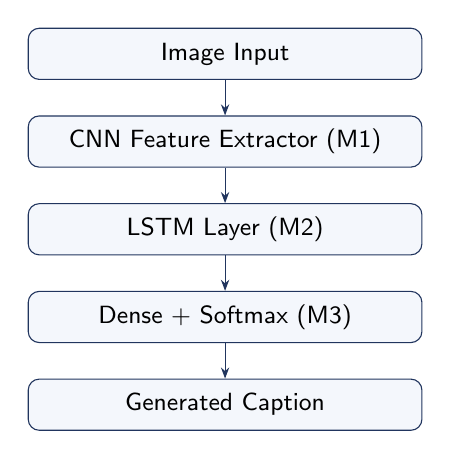
\begin{tikzpicture}[
  node distance=0.45cm,
  block/.style={draw=navy, rounded corners, fill=intuFill,
                minimum width=5cm, minimum height=0.65cm,
                font=\sffamily\small, align=center}
]
  \node[block] (img)   {Image Input};
  \node[block, below=of img]   (cnn)  {CNN Feature Extractor (M1)};
  \node[block, below=of cnn]   (lstm) {LSTM Layer (M2)};
  \node[block, below=of lstm]  (dns)  {Dense + Softmax (M3)};
  \node[block, below=of dns]   (cap)  {Generated Caption};
  \foreach \a/\b in {img/cnn,cnn/lstm,lstm/dns,dns/cap}
    \draw[-{Stealth[length=4pt]},navy] (\a) -- (\b);
\end{tikzpicture}
\end{center}

\medskip
This structure was not manually designed.
Evolution assembled it.
\end{worked}

\begin{worked}{Step 3 --- Fitness evaluation}
Train each assembled network for a few epochs.
Score each with the \vocab{BLEU score}.
BLEU runs from 0 to 1 and measures how well a caption matches a reference.
Higher is better.

\begin{center}\small
\begin{tabular}{@{}ccc@{}}
\toprule
\textbf{Network} & \textbf{BLEU Score} & \textbf{Fitness} \\
\midrule
N1 & 0.71 & 0.71 \\
N2 & 0.88 & 0.88 \\
N3 & 0.64 & 0.64 \\
\bottomrule
\end{tabular}
\end{center}

Best network this generation: $N2 = 0.88$.
\end{worked}

\begin{worked}{Step 4 --- Fitness-proportionate selection}
We use roulette-wheel selection.
Each network's chance equals its fitness divided by total fitness.

\begin{steps}
  \item \textbf{Total fitness.}
        \[ T = 0.71 + 0.88 + 0.64 = 2.23 \]

  \item \textbf{Selection probabilities.}
        \begin{align*}
          P(N1) &= 0.71 / 2.23 = \mathbf{0.318} \\
          P(N2) &= 0.88 / 2.23 = \mathbf{0.394} \\
          P(N3) &= 0.64 / 2.23 = \mathbf{0.287}
        \end{align*}

  \item \textbf{Select parents.}
        $N2$ has the highest probability.
        $N1$ has the second highest.
        They become parents for crossover.

  \item \textbf{Sense-check.}
        Sum: $0.318 + 0.394 + 0.287 = 0.999 \approx 1.0$. Good.
        Better networks get a bigger slice of the wheel.
\end{steps}
\end{worked}

\begin{worked}{Step 5 --- Crossover}
Parent architectures:
\[
  \text{Parent 1 (N2):}\quad \text{CNN} \to \text{LSTM} \to \text{Dense}
\]
\[
  \text{Parent 2 (N1):}\quad \text{CNN} \to \text{CNN} \to \text{Dense}
\]

Apply one-point crossover after the first module.

\begin{steps}
  \item \textbf{Split each parent after module 1.}
        P1 prefix: [CNN]; P1 suffix: [LSTM $\to$ Dense].
        P2 prefix: [CNN]; P2 suffix: [CNN $\to$ Dense].

  \item \textbf{Swap suffixes.}
        \begin{align*}
          \text{Child 1:} & \quad \text{CNN} \to \text{CNN} \to \text{Dense} \\
          \text{Child 2:} & \quad \text{CNN} \to \text{LSTM} \to \text{Dense}
        \end{align*}

  \item \textbf{Interpret.}
        Child 1 has two CNN stages (deeper feature extraction).
        Child 2 uses CNN then LSTM (feature extraction then sequence
        modelling).
\end{steps}
\end{worked}

\begin{worked}{Step 6 --- Mutation}

\begin{steps}
  \item \textbf{Mutate Child 1.}
        Change the second CNN's filter size from $3\times3$ to $5\times5$:
        \[
          \text{Child 1 after:}\quad
          \text{CNN}(3\times3) \to \text{CNN}(5\times5) \to \text{Dense}
        \]
        Larger filters capture broader patterns such as full face regions.

  \item \textbf{Mutate Child 2.}
        Increase the LSTM hidden size to 256 neurons:
        \[
          \text{Child 2 after:}\quad
          \text{CNN} \to \text{LSTM}(256) \to \text{Dense}
        \]
        More LSTM neurons improve sequence memory for caption generation.

  \item \textbf{Next generation population.}
        \begin{center}\small
        \begin{tabular}{@{}ll@{}}
        \toprule
        \textbf{Network} & \textbf{Architecture} \\
        \midrule
        Parent N1  & CNN $\to$ LSTM $\to$ Dense \\
        Parent N2  & CNN $\to$ CNN $\to$ Dense \\
        Child 1    & CNN($3\times3$) $\to$ CNN($5\times5$) $\to$ Dense \\
        Child 2    & CNN $\to$ LSTM(256) $\to$ Dense \\
        \bottomrule
        \end{tabular}
        \end{center}
\end{steps}
\end{worked}

\begin{worked}{Step 7 --- Next-generation fitness evaluation}
Train and evaluate all four networks again.

\begin{center}\small
\begin{tabular}{@{}lc@{}}
\toprule
\textbf{Network} & \textbf{Accuracy} \\
\midrule
Parent N1       & 88\% \\
Parent N2       & 84\% \\
Mutated Child 1 & 91\% \\
Mutated Child 2 & \textbf{94\%} \\
\bottomrule
\end{tabular}
\end{center}

Mutated Child 2 (CNN $\to$ LSTM(256) $\to$ Dense) is now the best
architecture.
The LSTM size increase improved sequence learning.
Evolution found this without any human decision.
\end{worked}

% =============================================================================
\section{The full CoDeepNEAT pipeline: cat vs.\ dog classification}
% =============================================================================

The slides also trace what each layer does inside an evolved network
for image classification.

\subsection{Input as numbers}

A $32\times32$ colour image has $32 \times 32 \times 3 = 3072$ values.
Each pixel has three channels (R, G, B), each from 0 to 255.
Normalize to $[0, 1]$ by dividing by 255.
Example: pixel $(120, 80, 60) \to (0.47, 0.31, 0.23)$.
At this point the system sees only numbers, not a cat.

\subsection{The evolved architecture}

CoDeepNEAT evolved these modules (not chosen by any human):
\begin{itemize}
  \item Module 1: Conv($3\times3$) + ReLU
  \item Module 2: Conv($5\times5$) + Pool
  \item Module 3: Dense layer
\end{itemize}

% CoDeepNEAT evolved architecture pipeline for cat/dog classification
\begin{figure}[htbp]
\centering
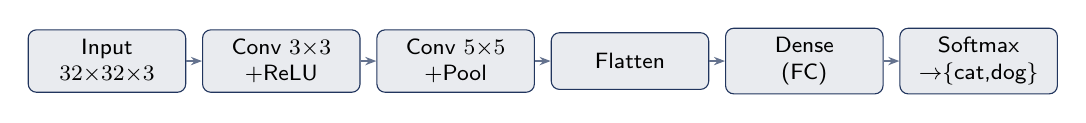
\begin{tikzpicture}[
  node distance=0.55cm and 0.2cm,
  blk/.style={rectangle,rounded corners=3pt,draw=navy,fill=navy!10,
              minimum width=2.0cm,minimum height=0.72cm,
              font=\footnotesize\sffamily,align=center},
  arr/.style={-{Stealth[length=4pt]},thick,color=navy!70}
]
  \node[blk] (inp) {Input\\$32{\times}32{\times}3$};
  \node[blk,right=of inp] (c1)  {Conv $3{\times}3$\\+ReLU};
  \node[blk,right=of c1]  (c2)  {Conv $5{\times}5$\\+Pool};
  \node[blk,right=of c2]  (flat){Flatten};
  \node[blk,right=of flat](fc)  {Dense\\(FC)};
  \node[blk,right=of fc]  (sm)  {Softmax\\$\to$\{cat,dog\}};

  \draw[arr] (inp)  -- (c1);
  \draw[arr] (c1)   -- (c2);
  \draw[arr] (c2)   -- (flat);
  \draw[arr] (flat) -- (fc);
  \draw[arr] (fc)   -- (sm);
\end{tikzpicture}
\caption*{\small\color{mutedtext}The CoDeepNEAT-evolved pipeline for cat vs.\ dog: two convolution modules (evolved) feed a dense classifier ending in a two-class softmax.}
\end{figure}

\subsection{What each layer does}

\begin{description}[leftmargin=7em,style=nextline,font=\normalfont\bfseries\color{navy}]
  \item[Conv $3\times3$] Applies a $3\times3$ filter.
    Detects edges: ears, body outlines.
    Outputs a feature map highlighting edges.
  \item[ReLU] $f(x) = \max(0, x)$.
    Removes negative values.
    Keeps only strong, positive edge responses.
  \item[Conv $5\times5$] Combines edges into textures: fur patterns,
    eye regions.
    Now the network distinguishes cat-like from dog-like texture.
  \item[Max Pool $2\times2$] Reduces spatial size.
    Keeps the strongest value in each $2\times2$ block.
    Answers ``Is the feature present?'' not ``Where exactly?''
  \item[Dense] Combines textures into parts: triangular ears, small
    nose, whisker lines.
  \item[Flatten + Dense] Flattens all features to a vector.
    Learns rules like ``whiskers + triangular ears = likely cat.''
\end{description}

\subsection{Softmax output}

The softmax function turns raw scores (logits) into probabilities.
For class $y_i$ with raw score $z_i$:

\begin{equation}
  P(y_i) = \frac{e^{z_i}}{\displaystyle\sum_j e^{z_j}}
\end{equation}

\noindent Suppose cat logit $= 2.5$ and dog logit $= 0.3$:
\begin{align}
  e^{2.5} &= 12.18, \quad e^{0.3} = 1.35 \\
  P(\text{cat}) &= \frac{12.18}{12.18 + 1.35} = \frac{12.18}{13.53} \approx 0.90 \\
  P(\text{dog}) &= \frac{1.35}{13.53} \approx 0.10
\end{align}

Final prediction: \textbf{Cat (90\% confidence)}.
(The slides use slightly different logits, giving 92\%.)

\subsection{Backpropagation when wrong}

If the true label is Dog but the prediction is Cat, the error is:
\[
  \text{Loss} = \text{cross-entropy}\bigl(-\log P(\text{dog})\bigr)
\]
Gradient descent updates all weights to reduce this loss.
Over many training images the weights converge so the network
classifies correctly.

\textbf{Where this shows up in ML.}
This layer hierarchy is the foundation of every CNN: ResNet, VGG,
EfficientNet.
CoDeepNEAT automates the choice of which layers to use and how to
connect them, removing the need for manual architecture design.

\begin{watchout}
The network does not see animals the way humans do.
It processes edges, then textures, then parts, then a label.
A cleverly crafted adversarial input can fool it by tweaking a few
pixels while still looking normal to a human eye.
\end{watchout}

% =============================================================================
\section{Comparison: NEAT, DeepNEAT, and CoDeepNEAT}
% =============================================================================

\begin{adjustbox}{max width=\linewidth}
\begin{tabular}{@{}p{3cm}p{3.3cm}p{3.3cm}p{3.6cm}@{}}
\toprule
\textbf{Property} & \textbf{NEAT} & \textbf{DeepNEAT} & \textbf{CoDeepNEAT} \\
\midrule
Node represents & single neuron & one full layer & module species (placeholder) \\
Evolves weights & yes & no (gradient descent) & no (gradient descent) \\
Handles deep CNNs & no & yes (unstructured) & yes (structured, modular) \\
Reuses components & no & no & yes (modules reused across blueprint) \\
Two co-evolving populations & no & no & yes (blueprints + modules) \\
Main use & small control tasks & medium-depth nets & large structured deep networks \\
\bottomrule
\end{tabular}
\end{adjustbox}

% =============================================================================
\section*{Glossary \& symbols}
\addcontentsline{toc}{section}{Glossary \& symbols}
% =============================================================================

\noindent\textbf{Key terms.}
\begin{description}[leftmargin=9em,style=nextline,font=\normalfont\bfseries\color{navy}]
  \item[ACO] Ant Colony Optimization; simulated ants deposit pheromone
    to guide search toward good solutions.
  \item[TSP] Travelling Salesman Problem; find the shortest tour visiting
    every city exactly once.
  \item[pheromone] Digital scent on a graph edge; accumulates on good
    paths and evaporates over time.
  \item[evaporation] The decay of pheromone each iteration; prevents
    locking onto a suboptimal route early.
  \item[NTP] Next Transition Probability; the formula an ant uses to pick
    its next city.
  \item[NAS] Neural Architecture Search; automated search for the best
    neural network structure.
  \item[NEAT] NeuroEvolution of Augmenting Topologies; evolves neural
    network topology using genetic algorithms.
  \item[innovation number] A unique ID for each structural mutation;
    ensures correct alignment during crossover.
  \item[speciation] Grouping similar architectures so they compete within
    their group, preserving diversity.
  \item[DeepNEAT] NEAT extended so each graph node is a full layer,
    not a single neuron.
  \item[CoDeepNEAT] Co-evolving Deep NEAT; splits architecture into
    blueprints (structure) and modules (reusable sub-networks).
  \item[blueprint] High-level graph in CoDeepNEAT; each node is a module
    species placeholder.
  \item[module] A small reusable sub-network in CoDeepNEAT; defines layer
    types and hyperparameters.
  \item[phenotype] The actual trainable network assembled from a blueprint
    and a set of modules.
  \item[fitness] A score measuring how well a network performs; drives
    selection.
  \item[shared fitness] Distributes a network's fitness score back to
    both the blueprint and all participating modules.
  \item[BLEU score] A metric for text generation quality (0 to 1);
    higher is better.
  \item[ReLU] Rectified Linear Unit; $f(x) = \max(0, x)$.
  \item[softmax] Turns a vector of raw scores into probabilities summing
    to 1.
\end{description}

\medskip
\noindent\textbf{Symbols at a glance.}
\begin{center}\small
\begin{tabular}{@{}p{2.8cm}p{9.5cm}@{}}
\toprule
\textbf{Symbol} & \textbf{Meaning} \\
\midrule
$N$              & Number of ants (must be $> 1$) \\
$\tau_{ij}$      & Pheromone on edge $(i,j)$; higher $=$ more attractive \\
$\tau_0$         & Initial pheromone level, usually 0 \\
$\eta_{ij}$      & Heuristic on edge $(i,j)$; $= 1/d_{ij}$ (inverse distance) \\
$\alpha$         & Weight given to pheromone in NTP \\
$\beta$          & Weight given to heuristic (distance) in NTP \\
$\rho$           & Evaporation coefficient; $0 < \rho < 1$ \\
$Q$              & Pheromone deposit constant \\
$f_k$            & Tour cost of ant $k$; shorter tours get higher reward \\
$\Delta\tau_{ij}^k$ & Pheromone deposited by ant $k$ on edge $(i,j)$; $= Q/f_k$ if used \\
$NTP_{ij}$       & Probability of ant moving from city $i$ to city $j$ \\
$P(y_i)$         & Softmax probability of class $y_i$ \\
$z_i$            & Logit (raw score) for class $i$ before softmax \\
\bottomrule
\end{tabular}
\end{center}

\end{document}
